%%%%%%%%%%%%%%%%%%%%%%%%%%%%%%%%%%%%%%%%%%%%%%%%%%%%%%%%%%%%%%%%%
% Dissertacao de Mestrado / Dept Fisica, CFM, UFSC              %
% Andre@UFSC - 2011                                             %
%%%%%%%%%%%%%%%%%%%%%%%%%%%%%%%%%%%%%%%%%%%%%%%%%%%%%%%%%%%%%%%%%

%:::::::::::::::::::::::::::::::::::::::::::::::::::::::::::::::%
%                                                               %
%                          Capítulo 2                           %
%                                                               %
%:::::::::::::::::::::::::::::::::::::::::::::::::::::::::::::::%

%***************************************************************%
%                                                               %
%                            Galex                              %
%                                                               %
%***************************************************************%

\chapter{O {\em Galaxy Evolution Explorer} (\galex)}
\label{sec:Galex}


%***************************************************************%
%                                                               %
%                     Galex - Objetivos                         %
%                                                               %
%***************************************************************%

\section{Objetivos do \galex}
\label{sec:Galex:Objetivos}

O {\em Galaxy Evolution Explorer} (\galex) é um telescópio espacial de pequeno
porte da NASA\footnote{{\em NASA Small Explorer} ({\em SMEX}) -
\url{http://explorers.gsfc.nasa.gov/missions.html}}, lançado em 28 de abril de
2003 para conduzir um {\em survey} de todo o céu numa faixa espectral do
ultravioleta ($1350$--$2750$\AA). O objetivo principal do \galex é estudar a
evolução da taxa de formação estelar em galáxias \citep{Martin2005}. Os dados
coletados pela missão são publicados em {\em Data Releases} periódicos,
denominados {\em General Releases}. Este trabalho foi realizado sobre os dados
do sexto {\em General Release}, GR6.

A missão consiste em uma série de {\em surveys} fotométricos e espectroscópicos
(ver tabela \ref{tab:GalexSurveys}). Destes, os principais {\em surveys} são o
{\em All Sky Survey} (AIS) e o {\em Medium Imaging Survey} (MIS), que foram
utilizados neste trabalho. O imageamento é feito em duas bandas espectrais:
ultravioleta distante ({\em far ultraviolet}, FUV), de $1350$ a $1750$\AA, e
ultravioleta próximo ({\em near ultraviolet}, NUV), de $1750$ a $2750$\AA. As
curvas de transmissão dos filtros utilizados nessas bandas podem ser visto na
figura \ref{fig:GalexFilters}. A espectroscopia é feita inserindo-se no caminho
ótico um {\em grism}, que consiste num prisma combinado com uma rede de
difração. Obtém-se deste modo um espectro de baixa resolução para cada objeto na
imagem, conforme descrito por \citet{Morrissey2007}.

\begin{table}
	\caption[{\em Surveys} realizados pelo \galex.]{{\em Surveys} realizados pelo
	\galex. O CAI consiste em observações de anãs brancas para calibração. A
	cobertura do céu é dada em graus quadrados. No caso do NGS, a magnitude limite
	é dada em unidades de densidade superficial de magnitude. Informações retiradas
	de \citet{Martin2005}.}
	\begin{tabular}{l r r}
		{\em Survey} & Cobertura do céu & Mag. AB limite \\ 
		\midrule
		{\em Calibration Imaging (CAI)}              &       - &            - \\
		{\em All-sky Imaging Survey (AIS)}           & $26000$ &       $20.5$ \\
		{\em Medium Imaging Survey (MIS)}            &  $1000$ &         $23$ \\
		{\em Deep Imaging Survey (DIS)}              &    $80$ &         $25$ \\
		{\em Nearby Galaxy Survey (NGS)}             &    $80$ &       $27.5$ \\
		{\em Wide Field Spectroscopic Survey (WSS)}  &    $80$ &         $20$ \\
		{\em Medium-deep Spectroscopic Survey (MSS)} &     $8$ & $21.5$--$23$ \\
		{\em Deep Spectroscopic Survey (DSS)}        &     $2$ &   $23$--$24$ \\
	\end{tabular}
	\label{tab:GalexSurveys}
\end{table}

\begin{figure}
	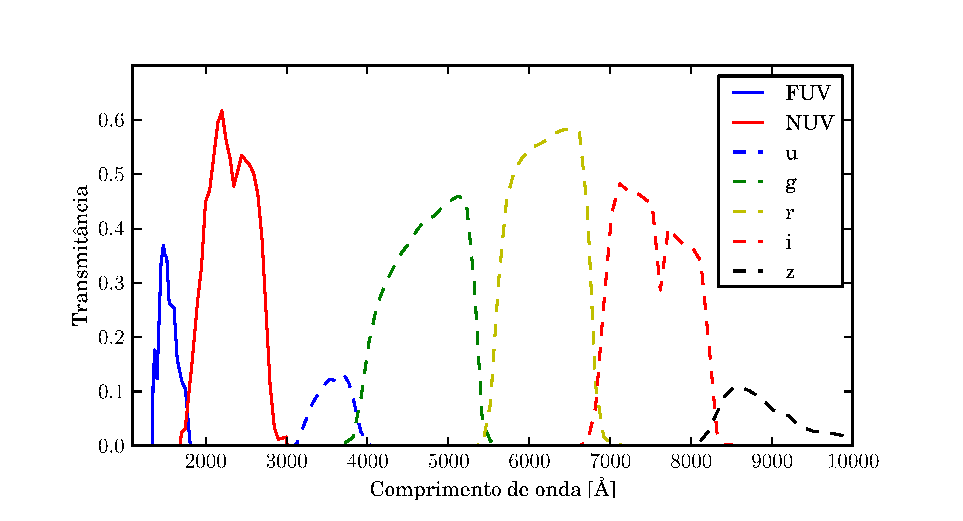
\includegraphics{figuras/galex-filters.eps}
	\caption[Curvas de transmissão dos filtros do \galex.]
	{Curvas de transmissão dos filtros do \galex, medidas em
	laboratório \citep{Morrissey2005}. Retirada do {\em website} mantido por
	Peter Capak: \url{http://www.astro.caltech.edu/~capak/cosmos/filters/}}
	\label{fig:GalexFilters}
\end{figure}

Os {\em surveys} do \galex foram planejados de forma a se valer de outros {\em
surveys} já existentes em outros comprimentos de onda. A figura
\ref{fig:GalexSDSSOverlap} mostra a sobreposição da área observada
\footnote{{\em Footprint}, no linguajar astronômico.} pelos {\em surveys} AIS e
MIS do \galex e do {\em Sloan Digital Sky Survey} (\SDSS). O objetivo primário da
missão do \galex é calibrar da taxa de formação estelar no universo local e a
determinar o histórico cosmológico de formação estelar entre os {\em redshifts}
$0 < z < 2$ \citep{Martin2005}. A comparação com dados de {\em surveys} em outros
comprimentos de onda tem um papel fundamental no cumprimento deste objetivo.

\begin{figure}
	\includegraphics[width=1.0\columnwidth]{figuras/footprint.eps}
	\caption[{\em Footprint} dos {\em surveys} \galex AIS, MIS e SDSS]
	{{\em Footprint} dos {\em surveys} \galex GR2+3 AIS (azul), MIS (vermelho) e
	SDSS DR6 (verde), de \citet{Budavari2009}}
	\label{fig:GalexSDSSOverlap}
\end{figure}


%***************************************************************%
%                                                               %
%                Galex - O céu no ultravioleta                  %
%                                                               %
%***************************************************************%

\section{Histórico do estudo do céu no ultravioleta}
\label{sec:Galex:CeuUV}

% FIXME: Usar referência de livro-texto para céu UV.
A camada de ozônio, tão desejável pela proteção que oferece aos seres vivos,
cobra a sua taxa na astronomia. Observações na banda ultravioleta precisam ser
feitas fora da atmosfera terrestre, portanto não é de se estranhar que o
trabalho nesta faixa espectral tenha progredido menos do que na faixa do óptico
e do infravermelho.\citneed

O primeiro trabalho sistemático de observação UV foi feito pelo {\em Orbiting
Astronomical Observatory 2} \citep{Code1970}, obtendo fotometria e
espectroscopia de estrelas brilhantes, aglomerados globulares e galáxias
próximas. Durante as décadas de 1970 e 1980, este e outros satélites como o TD-1
\citep{Boksenberg1973}, o {\em Astronomical Netherlands Satellite}
\citep{vanDuinen1975} e o {\em International Ultraviolet Explorer}
\citep{Kondo1987} -- o primeiro satélite a utilizar um detetor de imageamento UV
-- forneceram os dados fundamentais para os modelos de síntese de população
estelar de galáxias. {\em Surveys} de campo amplo foram feitos por uma câmera
lunar erguida por astronautas da {\em Apollo 16} \citep{Carruthers1973}, a bordo
do {\em Skylab} \citep{Henize1975} e pelo instrumento {\em FAUST} a bordo do
{\em Spacelab} \citep{Bowyer1993}. Muitas imagens UV também foram obtidas pelo
{\em Ultraviolet Imaging Telescope} em duas missões em ônibus espacial
\citep{Stecher1997}.


%***************************************************************%
%                                                               %
%                     Galex - Resultados obtidos                %
%                                                               %
%***************************************************************%

\section{Resultados obtidos pelo \galex}
\label{sec:Galex:Resultados}

o \galex fez o primeiro {\em survey} do céu inteiro em UV. As regiões próximas
ao plano da Galáxia foram evitados para não danificar os detetores. Pode-se ter
uma idéia do sucesso desta missão considerando a grande quantidade de artigos
publicados\footnote{Há uma lista com as mais de 500 publicações relacionadas ao
projeto do \galex em
\url{http://www.galex.caltech.edu/researcher/publications.html}}. Abaixo segue
um resumo dos resultados mais notáveis.

\citet{Wyder2007} analisam a distribuição de galáxias em função da cor UV e da
magnitude absoluta no universo local. Esta distribuição é conhecida como {\em
Diagrama Cor--Magnitude} (CMD, na sigla em inglês para {\em Color-Magnitude
Diagram}). Os autores usam {\em redshifts} e fotometria óptica obtidas do \SDSS
junto com fotometria UV do {\em survey} MIS do \galex. A amostra do \SDSS é
correlacionada com a do \galex procurando o objeto do \galex mais próximo de
cada objeto \SDSS até um limite de $4$'' ($4$ segundos de arco).

O diagrama cor-magnitude elaborado por \citeauthor{Wyder2007} mostra a separação
das galáxias nas sequências azul e vermelha (figura \ref{fig:WyderCMD}). Esta
distribuição bimodal é um resultado bem conhecido na astronomia.\citneed Porém,
diferente do diagrama cor-magnitude para a faixa espectral do óptico, a
distribuição de cores em UV não pode ser ajustada somente pela soma de duas
gaussianas, há um excesso de objetos nas cores intermediárias entre os picos
azul e vermelho. A boa separação entre as sequências é atribuída a uma maior
sensibilidade à formação estelar recente.

\begin{figure}
	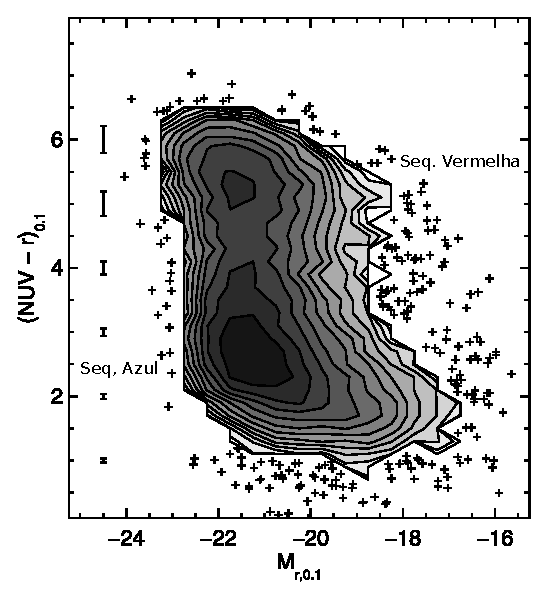
\includegraphics[width=0.7\columnwidth]{figuras/cmd-wyder.eps}
	\caption[Diagrama cor-margnitude em ultravioleta.]
	{Diagrama cor-margnitude em ultravioleta. \citep[figura 7]{Wyder2007}.}
	\label{fig:WyderCMD}
\end{figure}

\citet{Martin2007} investigaram as propriedades das galáxias entre as sequências
vermelha e azul para a mesma amostra citada acima. As galáxias nesta região
intermediária são preferencialmente galáxias com núcleo ativo ({\em Active
Galactic Nucleus}, AGN). Os autores estimam o fluxo de massa de galáxias indo da
sequência azul para a vermelha.

% FIXME: O que é a função de luminosidade para o univeso local? Entender o que
% isto significa.
Ainda para a mesma amostra, \citet{Schiminovich2007} investigaram a correlação
entre a morfologia das galáxias e a sua posição no CMD. A função de luminosidade
UV do universo local é medida -- pela primeira vez, segundo os autores -- com
relação aos parâmetros estruturais e à inclinação das galáxias.

% FIXME: Referência para a missão Kepler.
A missão do \galex se encerra em 31 de dezembro de 2011. Dados coletados após o
GR6, como as observações no mesmo campo utilizado na missão Kepler
\citep{KeplerMission}, observações de M31 e da Nuvem de Magalhães, entre outros,
serão liberados num último {\em data release}, GR7. Os dados obtidos pelo \galex
permanecerão disponíveis publicamente no MAST.



%***************************************************************%
%                                                               %
%                     Galex - Banco de dados                    %
%                                                               %
%***************************************************************%

\section{Data releases e banco de dados}
\label{sec:Galex:BancoDeDados}

% FIXME: Arrumar uma tradução melhor para ``tile''.
Os dados obtidos pelo \galex são armazenados no {\em Multi-Mission archive at
the Space Telescope Science Institute} (MAST). O acesso a estes dados é público,
a liberação é feita anualmente em {\em General Releases} (GR). Os dados
consistem basicamente em imagens e catálogos, divididos em campos ({\em tiles})
com área de aproximadamente $1,2$ graus quadrados. Devido ao modo como o \galex
faz as observações, um determinado objeto pode estar presente em mais de um
campo. A tabela \ref{tab:GalexReleases} mostra o número cumulativo de campos
observados por {\em survey} em cada GR\footnote{Informações retiradas do {em
website} do GR6: \url{http://galex.stsci.edu/GR6/}}. Observações de
pesquisadores convidados ({\em Guest Investigators}, GI) foram selecionadas de
forma a complementar os {\em surveys}.

\begin{table}
	\caption[Campos observados em cada {\em General Release} do \galex.]{Campos
	observados em cada {\em General Release} do \galex.}
	\begin{tabular}{l r r r r r r r r}
		{\em Release} & AIS   & DIS & MIS  & NGS & GI   & CAI & Espectros & Total \\
		\midrule
		GR1           & 3074  & 14  & 112  & 52  & -    & -   & 7         & 3259  \\
		GR2/GR3       & 15721 & 165 & 1017 & 296 & 288  & 20  & 41        & 17548 \\
		GR4/GR5       & 28269 & 292 & 2161 & 458 & 788  & 38  & 174       & 32180 \\
		GR6           & 28889 & 338 & 3479 & 480 & 1314 & 51  & -         & 34551 \\
	\end{tabular}
	\label{tab:GalexReleases}
\end{table}

Para facilitar o acesso aos dados do \galex, o MAST desenvolveu uma ferramenta
chamada {\em GalexView}, utilizando tecnologia {\em Adobe Flex}\footnote{{\em
Adobe Flex} é um {\em framework} de código aberto que permite desenvolver
aplicações para {\em web browsers}. Ver
\url{http://www.adobe.com/products/flex.html}.}. Desta forma o {\em GalexView }
pode ser acessado através de seu {\em website}\footnote{GalexView:
\url{http://galex.stsci.edu/GalexView/}} em qualquer {\em web browser} que tenha
suporte ao {\em Adobe Flash Player}\footnote{{\em Adobe Flash Player} é uma
extensão multiplataforma para {\em web browsers} que provê capacidade de
visualização de conteúdo {\em flash} gerado tanto pelos seus editores
proprietários quanto por ferramentas de terceiros. Ver
\url{http://www.adobe.com/products/flashplayer/}.}.

Através do {\em GalexView} é possível fazer buscas, visualizar e obter imagens e
catálogos dos campos do \galex. As buscas podem ser feitas de forma bastante
versátil, tanto pelo nome do objeto quanto pelas coordenadas do céu. O formato
de entrada é flexível o suficiente para evitar os problemas causados por
idiossincrasias na notação de coordenadas (por exemplo, tanto ``14h03m12.6s
+54d20m56.7s'' quanto ``14 03 12.6 54 20 56.7'' ou ``210.83 54.35'' apontam para
a mesma região). A sua interface (figura \ref{fig:GalexView}) permite filtrar o
conteúdo retornado pelas buscas, separando por {\em surveys}. Há também uma
ferramenta de histograma, permitindo filtrar pelos valores das colunas dos
catálogos. Os objetos selecionados na busca aparecem marcados na visualização da
imagem. Utilizando um sistema do tipo ``carrinho de compras'', pode-se
selecionar campos e objetos de interesse, para ao final do uso do sistema baixar
toda a seleção de uma vez.

\begin{figure}
	\includegraphics[width=0.7\columnwidth]{figuras/galexview.eps}
	\caption[Tela do programa{\em GalexView}.]
	{Tela do programa {\em GalexView}, com a visualização da galáxia M101.}
	\label{fig:GalexView}
\end{figure}

Tanto o {\em GalexView} quanto outras ferramentas de busca do MAST, como o
\galex {\em Search Form} e o \galex {\em Tilelist}, são construídos sobre um
{\em banco de dados relacional} acessado através da linguagem {\em SQL}
\citep{Chamberlin1974}. Muito comum na indústria, bancos de dados relacionais
dispõem em geral de uma vasta gama de ferramentas para gerenciamento dos dados.
Uma de suas grandes vantagens é o uso de índices\footnote{Un índice numa tabela
de banco de dados é uma estrutura que copia partes da tabela numa determinada
ordem, de forma a aumentar a velocidade de acesso aos dados ao custo de espaço
de armazenamento.} para agilizar o acesso a dados. Embora a tecnologia exista
desde a década de 1970 \citep{Codd1970}, até uma década atrás suas vantagens
eram praticamente neglicenciadas na astronomia.

Bancos de dados relacionais e ferramentas para gerenciamento e acesso a dados
serão tratados com mais detalhes no capítulo \ref{sec:Crossmatch}.


% End of this chapter
